Dirbtiniai neuroniniai tinklai yra apmokomi naudojantis stochastiniu metodu, atsitiktinai pasirenkant pradinius svorius ir pateikiant apmokymo duomenis atsitiktine seka. Tad kiekvieną kartą apmokant tą patį dirbtinį neuroninį tinklą naudojant tuos pačius hiperparametrus, rezultatai skiriasi. Tad kuo daugiau kartų yra pakartotas tas pats tyrimas, tuo tiksliau yra atliekamas palyginimas. Šiame magistro baigiamajame darbe yra 10 kartų kartojami tyrimai renkant f1 įverčius su pilnomis apmokymo ir testavimo duomenų imtimis. Šiame kiekybiniame tyrime buvo renkami testavimo duomenų f1 įverčiai po kiekvieno pilno apmokymo.


Šio kiekybinio tyrimo rezultatai yra atvaizduoti blokinėse diagramose (angl. box plot). Blokinė diagrama - tai standartizuotas būdas pavaizduoti duomenų pasiskirstymą. Blokinėje diagramoje žalia linija kvadrato viduje žymi medianą (angl. median), kvadrato viršutinė briauna - viršutinį kvartilį (angl. quartile), o apatinė briauna - apatinį kvartilį. Linija virš kvadrato žymi maksimalią reikšmę atmetus kraštutines vertes (angl. outliers), paskaičiuojama pagal formulę $Q1 - 1.5 \times (Q3 - Q1)$, o linija po kvadratu - minimalią reikšmę atmetus kraštutines vertes, paskaičiuojama pagal formulę $Q3 + 1.5 \times (Q3 - Q1)$. Šiose formulėse $Q1$ yra apatinis kvartilis ir $Q3$ - viršutinis kvartilis. Galiausiai taškai blokinėse diagramose žymi kraštutines reikšmes.

Šios blokinės diagramos yra atvaizduotos \ref{img:box_weighted_f1} paveikslėlyje, \ref{img:box_micro_f1} paveikslėlyje ir \ref{img:box_macro_f1} paveikslėlyje, kur
mvcnn yra daugiavaizdžio konvoliucinio neuroninio tinklo f1 įverčiai, capsnet - kapsulinio neuroninio tinklo f1 įverčiai, 
mv\_cap\_capsnet1 - daugiavaizdžio kapsulinio neuroninio tinklo su vaizdų kapsuliniu sluoksniu ir vienu mokymosi etapu f1 įverčiai, 
mv\_cap\_capsnet2 - daugiavaizdžio kapsulinio neuroninio tinklo su vaizdų kapsuliniu sluoksniu ir dviem mokymosi etapais f1 įverčiai,
mv\_capsnet - daugiavaizdžio kapsulinio neuroninio tinklo su vaizdų sujungimo sluoksniu ir dviem mokymosi etapais f1 įverčiai.

\begin{figure}[H]
	\centering
	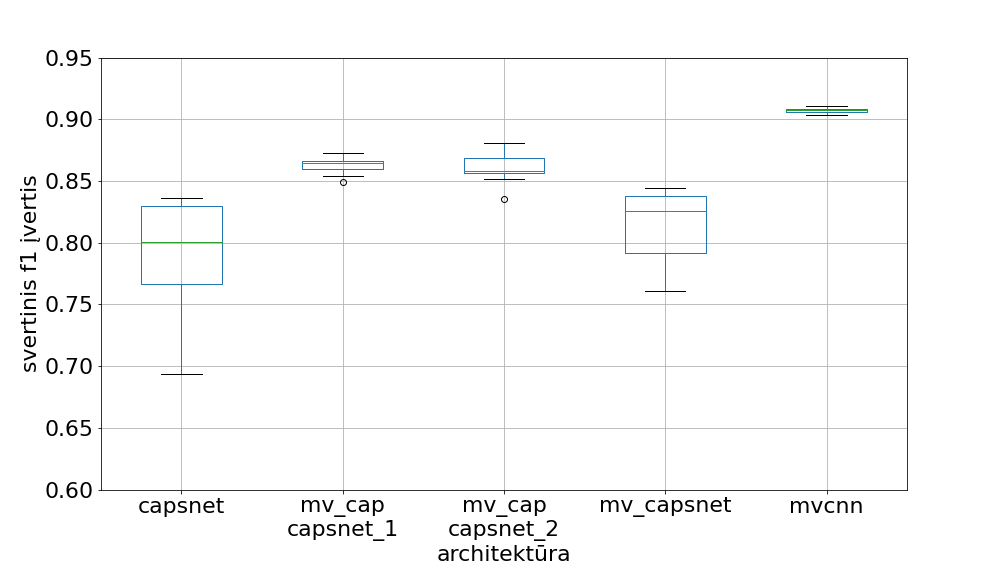
\includegraphics[scale=0.4]{img/boxplot_f1_weighted.png}
	\caption{
		Testavimo duomenų klasifikavimo svertiniai f1 įverčiai, kur mvcnn yra daugiavaizdžio konvoliucinio neuroninio tinklo f1 įverčiai, capsnet - kapsulinio neuroninio tinklo f1 įverčiai, mv\_cap\_capsnet1 - daugiavaizdžio kapsulinio neuroninio tinklo su vaizdų kapsuliniu sluoksniu ir vienu mokymosi etapu f1 įverčiai, mv\_cap\_capsnet2 - daugiavaizdžio kapsulinio neuroninio tinklo su vaizdų kapsuliniu sluoksniu ir dviem mokymosi etapais f1 įverčiai,
		mv\_capsnet - daugiavaizdžio kapsulinio neuroninio tinklo su vaizdų sujungimo sluoksniu ir dviem mokymosi etapais f1 įverčiai.
	}
	\label{img:box_weighted_f1}
\end{figure}

\begin{figure}[H]
	\centering
	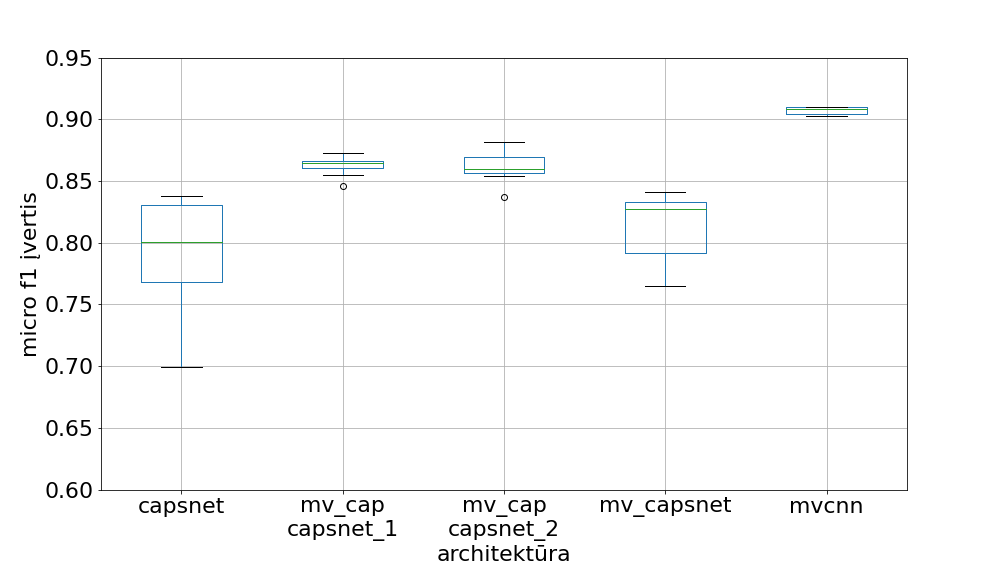
\includegraphics[scale=0.4]{img/boxplot_f1_micro.png}
	\caption{
		Testavimo duomenų klasifikavimo mikro f1 įverčiai, kur mvcnn yra daugiavaizdžio konvoliucinio neuroninio tinklo f1 įverčiai, capsnet - kapsulinio neuroninio tinklo f1 įverčiai, mv\_cap\_capsnet1 - daugiavaizdžio kapsulinio neuroninio tinklo su vaizdų kapsuliniu sluoksniu ir vienu mokymosi etapu f1 įverčiai, mv\_cap\_capsnet2 - daugiavaizdžio kapsulinio neuroninio tinklo su vaizdų kapsuliniu sluoksniu ir dviem mokymosi etapais f1 įverčiai,
		mv\_capsnet - daugiavaizdžio kapsulinio neuroninio tinklo su vaizdų sujungimo sluoksniu ir dviem mokymosi etapais f1 įverčiai.
	}
	\label{img:box_micro_f1}
\end{figure}

\begin{figure}[H]
	\centering
	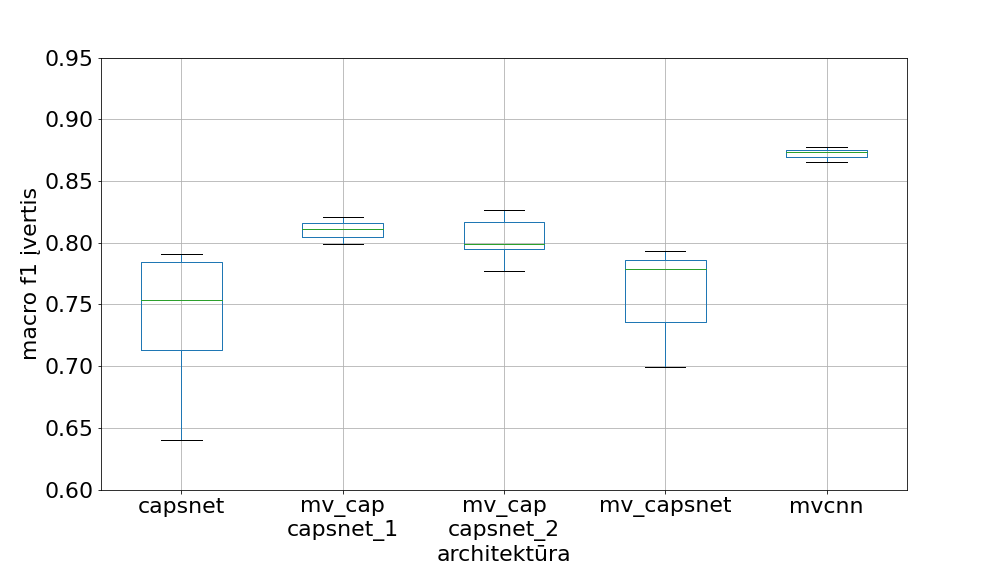
\includegraphics[scale=0.4]{img/boxplot_f1_macro.png}
	\caption{
		Testavimo duomenų klasifikavimo makro f1 įverčiai, kur mvcnn yra daugiavaizdžio konvoliucinio neuroninio tinklo f1 įverčiai, capsnet - kapsulinio neuroninio tinklo f1 įverčiai, mv\_cap\_capsnet1 - daugiavaizdžio kapsulinio neuroninio tinklo su vaizdų kapsuliniu sluoksniu ir vienu mokymosi etapu f1 įverčiai, mv\_cap\_capsnet2 - daugiavaizdžio kapsulinio neuroninio tinklo su vaizdų kapsuliniu sluoksniu ir dviem mokymosi etapais f1 įverčiai,
		mv\_capsnet - daugiavaizdžio kapsulinio neuroninio tinklo su vaizdų sujungimo sluoksniu ir dviem mokymosi etapais f1 įverčiai.
	}
	\label{img:box_macro_f1}
\end{figure}


\ref{img:box_weighted_f1} paveikslėlyje, \ref{img:box_micro_f1} paveikslėlyje ir \ref{img:box_macro_f1} paveikslėlyje pavaizduotos blokinės diagramos paneigia kai kurias įžvalgas padarytas iš \ref{img:train_plot} grafiko ir \ref{img:val_plot} grafiko. Iš šių blokinių diagramų matoma, kad daugiavaizdžio kapsulinio neuroninio tinklo su vaizdų kapsuliniu sluoksniu apmokymas vienu etapu pasiekia panašius klasifikavimo rezultatus kaip ir apmokymas dvejais etapais.

Taip pat \ref{img:box_weighted_f1} paveikslėlyje, \ref{img:box_micro_f1} paveikslėlyje ir \ref{img:box_macro_f1} paveikslėlyje pavaizduotos blokinės diagramos indikuoja, kad skirtumas tarp daugiavaizdžio kapsulinio neuroninio tinklo su vaizdų sujungimo sluoksniu ir kapsulinio neuroninio tinklo klasifikavimo rezultatų tikslumų skirtumas yra nereikšmingas.
